\documentclass{article}
\usepackage{color}
\usepackage{tikz}
\usepackage{float}
\usepackage{tabularx}
\usepackage{amsmath}
\usepackage{amssymb}
\usepackage{listings}
\usepackage{enumitem}
\usepackage{syntax}
\usepackage{csquotes}
\usepackage{pgfplots}
\usepackage{parskip}
\usepackage{fancyhdr}
\usepackage{vmargin}
\usepackage[backend=biber]{biblatex}
\addbibresource{references.bib}


\definecolor{dkgreen}{rgb}{0,0.6,0}
\definecolor{gray}{rgb}{0.5,0.5,0.5}
\definecolor{mauve}{rgb}{0.58,0,0.82}


\lstset{frame=tb,
  numbers=left,
  stepnumber=1,
  language=Java,
  aboveskip=3mm,
  belowskip=3mm,
  showstringspaces=false,
  columns=flexible,
  basicstyle={\small\ttfamily},
  numberstyle=\color{gray},
  keywordstyle=\color{blue},
  commentstyle=\color{dkgreen},
  stringstyle=\color{mauve},
  breaklines=true,
  breakatwhitespace=true,
  tabsize=2,
  moredelim=**[is][\color{red}]{@}{@},
}

\setlength{\grammarindent}{12em}

%\renewcommand{\lstlistingname}{Algorithm}
%\newcommand{\tablerow}[4]{ #1 & #2 & #3 & #4\\}
\newcommand{\n}[0]{\\[\baselineskip]}

%
% #1 - Module code
\newcommand{\maketitlepage}[2]{
\begin{titlepage}
	\centering
    
\includegraphics[scale = 0.4]{01-standard-vertical-black.png}\\	% University Logo
	\textsc{\LARGE #1}\\[0.5 cm]				% Course Code
	\rule{\linewidth}{0.2 mm} \\[0.4 cm]
	{ \huge \bfseries \thetitle}
	\rule{\linewidth}{0.2 mm} \\[0.5 cm]
	\textsc{\large \thedate}\\[1.5 cm]
	
	\begin{minipage}{0.4\textwidth}
		\begin{flushleft} \large
			\emph{Lecturer:}\\
			#2
			\end{flushleft}
			\end{minipage}~
			\begin{minipage}{0.4\textwidth}
            
			\begin{flushright} \large
			\emph{Submitted By:} \\
			\theauthor
		\end{flushright}
        
	\end{minipage}\\[2 cm]
	
\end{titlepage}
}

\title{Predicting energy use of appliances}
\author{140011146}

\makeatletter
\let\thetitle\@title
\let\theauthor\@author
\let\thedate\@date
\makeatother

\begin{document}


\maketitlepage{CS5014 Machine Learning}{David Harris-Birtill\\Kasim Terzi\'{c}}




\section{Introduction}
A paper \cite{paper} on prediction models of energy use of appliances using data gathered from a low energy house presented different prediction models to try and gain an understanding of appliance use in buildings. 
\n
As a machine learning exercise, the same raw dataset is taken and used to create a regression model. Each step of the machine learning methodology is carefully followed and documented to show off different consequences of decisions made. The resulting models are evaluated against test data and the results are discussed to see why a simple linear model is not a strong fit for the dataset.


\section{Data preprocessing}
The data preprocessing steps are first written in the python notebook as an example to show how that particular step works. Afterwords, before the start of choosing and training models, the preprocessing steps are written again as extensions to \texttt{sklearn}'s pipelines. This makes for a modular design as each step of the preprocessing process can be included or changed in the pipeline if tweaking is needed.
\subsection{Splitting test set}
Before even looking at the data, the first thing that was done was to split the data into training and test data. The test data will be put away until the end to run our different models on. This is to represent new unseen data, therefore we do not want to inspect at all so we can test how well our model performs against new data. This is why this splitting into test data is the very first thing that is done. The first decision is to decide the percentage split of training and test data. The percentage chosen represents a trade off between less training or less testing data.
\n
One disadvantage of splitting the data into training and test sets before looking at its contents is the risk of introducing sampling bias\cite{geron}. This is because the test set may not be representative of our dataset as the sampling is done completely randomly without taking into account different proportions of feature values. This may be fine on a larger dataset, but as our dataset is relatively small, it is a trade off we make for ensuring we don't introduce bias in our models from looking at the test data. Additionally, a validation set is not split again from the training data. This is done to keep all data for training due to the smaller dataset we have. Any parameter tuning or cross validation done is therefore done all on the training data. To counter the disadvantage of not having the separate validation set, k-fold cross validation is used.


\subsection{Data visualisation}

\subsubsection{Histograms}
We can visualise the data by plotting histograms of each column. This will tell us some information about how the data for each feature is distributed, and whether there might be errors in the data.

\begin{figure}[H]
\centering
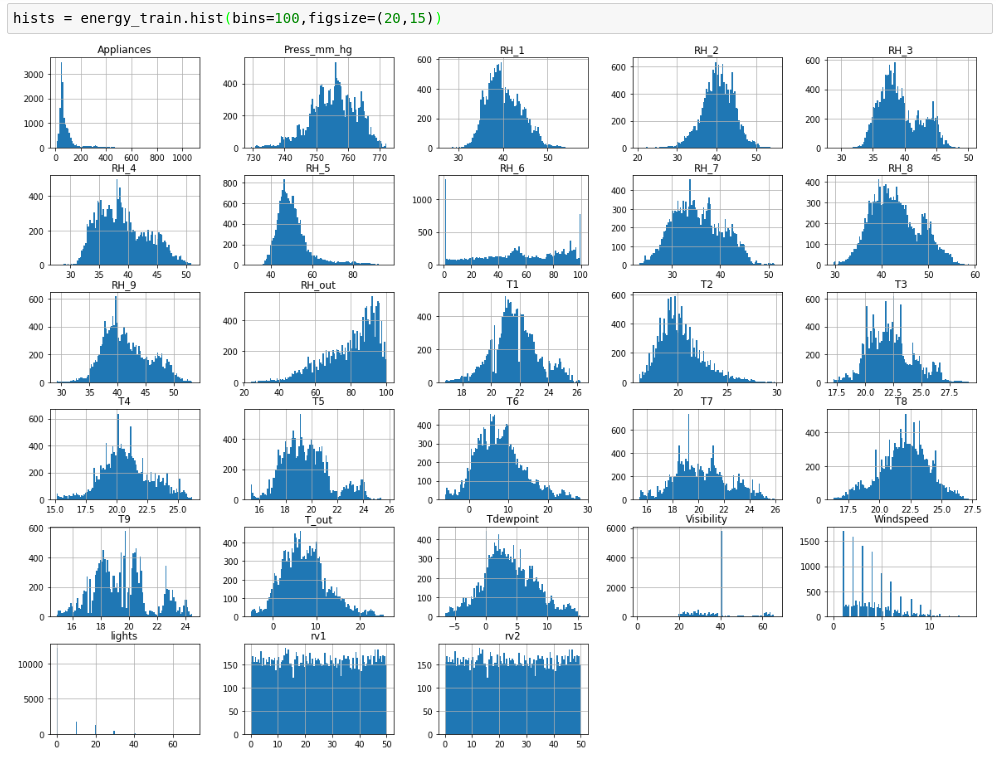
\includegraphics[width=1\textwidth, keepaspectratio]{imgs/histograms.png}
\caption{Histograms of all data features except for time.}
\end{figure}
\noindent
Time is not plotted here as we have not converted it from its string form yet. However, we expect the time to be quite regular, as the data is gathered as measurements after every certain timestamp over a period of 137 days. 
\n
We can see from the histograms, many of the temperature and relative humidity values follow a relatively normal distribution. Some features have very discrete values, for example the \textit{lights} feature only has a few unique values. There are also some features that don't follow a normal distribution. For example, the histogram for \textit{RH\_6} is interesting as it as many values at the extreme ends of the histogram. This is different from most of the other humidity sensors but can be explained because this is the one humidity sensor that was placed in the exterior of the house. Another example of an odd histogram is the \textit{Visibility}, as one value dominates compared to all others. Though this can be explained as the visibility being normal for most measurements and only changes rarely, it may not make for a good input feature as its values do not change very much.

\subsubsection{Temperature/Relative humidity correlation}

\begin{figure}[H]
\centering
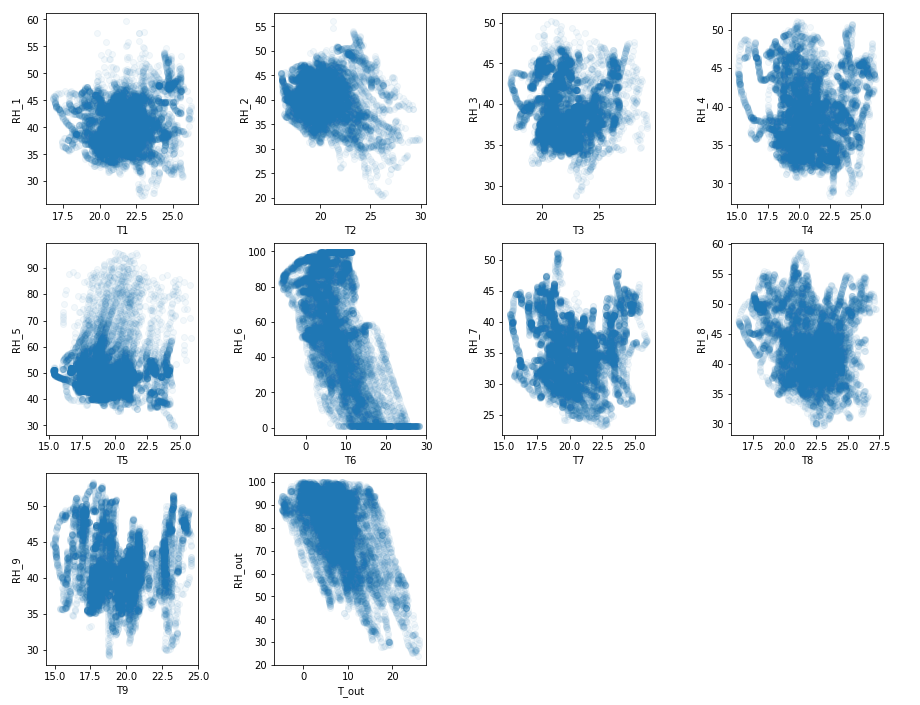
\includegraphics[width=1\textwidth, keepaspectratio]{imgs/t-rh-correlation.png}
\caption{Plotting each temperature measurement against the humidity of the same sensor to see if there is any correlation between the two.}
\end{figure}

TODO \cite{colinear}

\subsection{Data cleaning}
To clean the data, we must first observe what kind of data is given. From \cite{paper}, we know our data describes temperatures, relative humidity, energy consumption, pressure, windspeed, visibility and time. From knowledge of what the data represents, we can clean any values that don't make sense, for example negative humidity or extreme temperatures.
\n
From our visualisation, we can see in the histograms that there are no nonsensical values in our dataset, however, we cannot be sure this also applies to our unseen test data, so we should still include the cleaning step in our methodology, even if nothing is cleaned initially. Additionally, we can see there are no NaN or missing values from looking at the \texttt{pandas} dataframe, but we should still include a step for cleaning these values in case the test data has such values. 

\subsection{Converting datetime}
One column of the given data is a string timestamp, which includes the date and time the measurement was taken. 
\begin{lstlisting}[caption={Example timestamp snippet}, backgroundcolor = \color{lightgray}]
2016-01-26 12:30:00
\end{lstlisting}
In \cite{paper}, the time was converted into 3 input features: Number of seconds from midnight (NSM), Week status and Day of the week. The week status and day of the week were categorical features while number of seconds is numerical. However, these kind of features do not take into account the cyclical nature of time.
\n
To keep the cyclical nature of time, a different approach was used where the time of day and day of week features were created using a sine and cosine transform \cite{cyclic}. The use of the trigonometric functions keep the cyclical features, so for example 5 seconds before and after midnight would be represented as being 10 seconds apart rather than one being 5 seconds and the other being 86395 seconds. The sine and cosine features must be used together, as just using one of the two features gives a 12-hour representation rather than a full 24-hour representation. 



\subsection{Feature selection}
Now that we have prepared the inputs and converted the timestamp, we must choose a suitable subset of features of training. It is important to choose a strong features that help give better accuracy while removing unimportant features that may hurt the performance of the model. It is also better to have fewer features to keep the model simpler. It may help to improve the accuracy of some models and reduces computational requirements. Further, it would be easier to explain and understand a simple model compared to a very complex one. 
\n
The correlation between all features can be computed and visualised. The correlation is mapped to its absolute value, since negative correlation is just as strong as positive correlation only in the opposite direction. This lets us see if any pair of features are very strongly correlated and one could therefore be removed as it would be redundant. 

\begin{figure}[H]
\centering
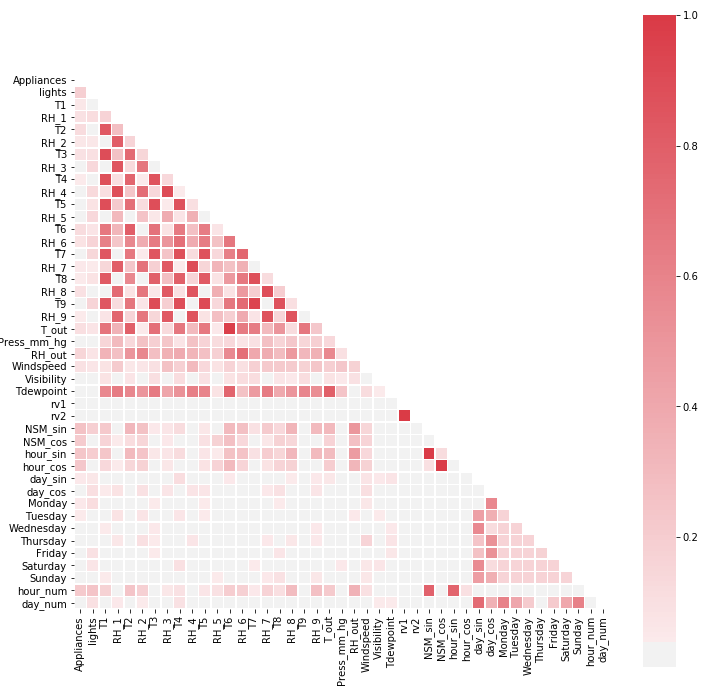
\includegraphics[width=1\textwidth, keepaspectratio]{imgs/all-corr.png}
\caption{Correlation matrix of all features in our dataset}
\end{figure}
\noindent
As we are wanting to use a linear model to begin with, the correlation between the input features and the output is quite important as that is how new output values will be predicted. Unfortunately, though many of the features correlate with each other, most have quite weak correlations with the output. From the correlation matrix, it is clear the random variables do not correlate to any of the other features except each other, so it would be important to remove them from our list of input features.  TODO


\subsubsection{Choosing date/time feature}
To choose which form to convert the timestamp to be, the correlation between each time feature and the output ``Appliances" features can also be computed. 
\begin{figure}[H]
\centering
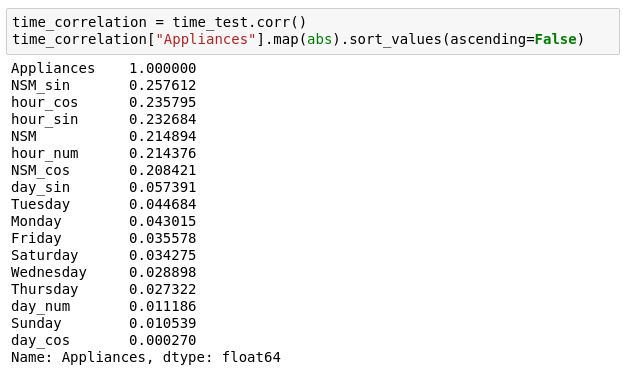
\includegraphics[width=0.7\textwidth, keepaspectratio]{imgs/time-correlation.png}
\caption{Correlation of different time input features against the output feature.}
\end{figure}
\noindent
We can see that the time of the day is a strong feature compared to the day of the week.  \texttt{hour\_sin} and \texttt{hour\_cos} was chosen as their correlation is better than \texttt{NSM} and \texttt{hour\_num}. They were chosen over \texttt{NSM\_sin} and \texttt{NSM\_cos} as \texttt{NSM\_cos} has a lower correlation but must be included if \texttt{NSM\_sin} is chosen. Our correlation matrix also shows that the cyclic \texttt{NSM} and cyclic hour values correlate strongly to each other, so only one of the two should be chosen as the other is redundant. 
\n
For the day of the week feature, we should again choose just one to avoid redundancy. The sine transformation of the day of the week is the most correlated to the output feature, however the cosine transform is not. Because of the consistency of the categorical features, it is chosen over the cyclical day of the week. 

\subsubsection{Feature selection algorithms}
We should also remove any input features with correlations less than that of the random variable. We can do this na\"{i}vely and keep all the rest of the input features, but we can also run some feature selection techniques to further reduce the number of input features.
\n
As \texttt{sklearn} provides various feature selection functions, some will be used in additional to our manual reduction of the feature set. 
\n
TODO different feature selection

\section{Model selection and training}
For the process of model selection, we first select a simple linear regression model. Then we add complexity to try and get less error by using ridge regression, then polynomial regression. The error values come from cross validating the trained model on the training data.
\n
After each model, the error is checked and a graph of the predicted values and true values is plotted to understand the reason behind the performance of the models.

\subsection{Model performance}
In general, the errors and results obtained had a similar performance to the results from \cite{paper}. Despite the different aspects to the input features and

\subsubsection{Linear regression}
First, we start with the simplest model of linear regression, training and k-fold cross validating on the training data. 
\n

TODO use learning curve to determine bias vs variance to see if underfit or overfit

\subsubsection{Polynomial regression}
As our first linear model does not seem to fit the data well, we can try using basis expansion with polynomial expansion to increase the variance of the model. 




We don't use regularisation models such as ridge regression or lasso regression as our model is underfitting, so suppressing our features with a reguarlisation parameter would do little to improve performance. We need to be able to better TODO

\section{Results and evaluation}

\section{Discussion}
From having used a few different regression methods to iteratively try and get a better model, it was found that (TODO) no model resulted in good performance on the dataset. From the graphs of the predicted values, we can see because we are using an underlying linear model, there are predicted values which are negative. This does not make sense in terms of what values we should be predicting, since the Wh of appliances cannot be negative. However, as a characteristic of linear models, it will not restrict the output from negative values, so perhaps a linear model is not suitable for this problem. 
\n
The residual graphs also give a clear trend, showing that as the actual value increases, the error increases as well.


\section{Conclusion}

https://www.analyticsvidhya.com/blog/2016/01/complete-tutorial-ridge-lasso-regression-python/

https://opendevincode.wordpress.com/2015/08/01/building-a-custom-python-scikit-learn-transformer-for-machine-learning/

https://github.com/ageron/handson-ml/blob/master/02_end_to_end_machine_learning_project.ipynb

\printbibliography

\end{document}



